\documentclass[fleqn]{article}
\usepackage[english]{babel}
\usepackage{a4wide}
\usepackage{latexsym}
\usepackage{times}
\usepackage{theorem}
\usepackage{url}
\usepackage[final]{graphics}
\usepackage{amsmath,amssymb}
\usepackage{amsfonts}
\usepackage{array}
\usepackage{calc}
\usepackage{xspace}
\usepackage{color}
\usepackage{epsfig}
\usepackage{subfigure}
\usepackage{float}
\usepackage{stmaryrd}
\usepackage{color}
\usepackage{mathtools}
\usepackage{graphicx}
\usepackage{epstopdf}
\usepackage{listings}
\usepackage{color}
\usepackage{booktabs,caption}
%\usepackage[flushleft]{threeparttable}

\DeclareMathAlphabet{\mathpzc}{OT1}{pzc}{m}{it}

\usepackage{amssymb}
\usepackage{graphicx}
\usepackage{epstopdf}
\usepackage{mathtools}

\usepackage{algorithm}
\usepackage[noend]{algpseudocode}

\usepackage{fouriernc}
\pagestyle{plain}
\usepackage{float}
\usepackage[hidelinks]{hyperref}

\usepackage{array}
\newcolumntype{L}[1]{>{\raggedright\let\newline\\\arraybackslash\hspace{0pt}}m{#1}}
\newcolumntype{C}[1]{>{\centering\let\newline\\\arraybackslash\hspace{0pt}}m{#1}}
\newcolumntype{R}[1]{>{\raggedleft\let\newline\\\arraybackslash\hspace{0pt}}m{#1}}

\newtheorem{theorem}{Theorem}
\newtheorem{fact}{Fact}
\newtheorem{hypothesis}{Hypothesis}
\newtheorem{lemma}{Lemma}
\newtheorem{definition}{Definition}

\definecolor{codegreen}{rgb}{0,0.6,0}
\definecolor{codegray}{rgb}{0.5,0.5,0.5}
\definecolor{codepurple}{rgb}{0.58,0,0.82}
\definecolor{backcolour}{rgb}{0.95,0.95,0.92}

\lstdefinestyle{mystyle}{
	backgroundcolor=\color{backcolour},   
	commentstyle=\color{codegreen},
	keywordstyle=\color{magenta},
	numberstyle=\tiny\color{codegray},
	stringstyle=\color{codepurple},
	basicstyle=\footnotesize,
	breakatwhitespace=false,         
	breaklines=true,                 
	captionpos=b,                    
	keepspaces=true,                 
	numbers=left,                    
	numbersep=5pt,                  
	showspaces=false,                
	showstringspaces=false,
	showtabs=false,                  
	tabsize=2
}

\lstset{style=mystyle}


\usepackage{fouriernc}
\pagestyle{plain}

%% macros.tex

\title{\sf Towards BCRT for FPTS}
\author{{\sf H.J. Rivera Verduzco 0977393}\\
{\footnotesize\sl P.O.~Box 513, 5600 MB Eindhoven, The Netherlands}\\
{\footnotesize \sl Email: \tt H.J.Rivera.Verduzco@student.tue.nl}}
%\date{}
\begin{document}
\maketitle

%\begin{abstract}
%\noindent
% Add abstract here %
%\end{abstract}

\section{Recap on initial results}
%The optimal instant as presented for FPPS occurs when the completion of a job of a task $\tau_i$ coincides with the simultaneous release of all its higher priority tasks. We now investigate whether this is a valid optimal instant for FPTS. For this case, consider the task-set $\mathpzc{T}_{\ref{tab:taskset2}}$ described in Table \ref{tab:taskset2}. Figure \ref{fig:bcrt2} shows an optimal instant of this task-set for task $\tau_3$ as described for FPPS. As can be seen, at the time $t=770$, the completion of task $\tau_3$ coincides with the release of higher priority tasks $\tau_1$ and $\tau_2$. The shortest response time for this situation, is $R_3=50$ and it is assumed by the job activated at time $t=610$. However, $R_3=50$ is an optimistic value for the \textit{best-case response time} under FPTS as we will show as follows. Figure \ref{fig:bcrt3} shows the same task-set $\mathpzc{T}_{\ref{tab:taskset2}}$ scheduled with different phases $\phi_i$. In this case, the \textit{shortest response time} for task $\tau_3$ is $R_3=30$, and it occurs at the time $t=630$. This response time coincides with the \textit{best-case execution time} $BC_3$; therefore, this is indeed the \textit{best-case response time}.

\begin{fact}
	In general, the optimal instant as presented for FPPS is not a valid optimal instant for FPTS.
\end{fact}

This fact illustrates the need of finding a generalized version of the optimal instant to find the \textit{best-case response time} under FPTS.

\begin{fact}
	Under FPTS, the shortest response time of a task $\tau_i$ in a level-$i$ active period is not necessarily assumed by the last job in that level-i active period.
\end{fact}

This fact illustrates that it is also necessarily to explore previous jobs in a level-i active period, not only the one experiencing the optimal instant.

\begin{fact}
	The best-case response time of a task $\tau_i$ can be affected by a higher priority task that cannot preempt $\tau_i$.
\end{fact}

This facts shows the importance of considering delaying tasks in the \textit{best-case response time analysis}

\begin{table}[H]
	\center
	\caption{Task set $\mathpzc{T}_{\ref{tab:taskset1}}$. The \textit{least common multiple} of the periods is 350.}
	\label{tab:taskset1}
	\begin{tabular}{c c c c c | c}
		\hline 
		& $T_i$ & $WC_i=BC_i$ & $\pi_i$ & $\theta_i$ &  $wl_i$\\ 
		\hline 
		$\tau_1$& 35 & 10  & 3 & 3 &  1\\ 
		$\tau_2$& 50 & 20  & 2 & 2 & 2 \\ 
		$\tau_3$& 70 & 22 & 1 & 2 & 5 \\
		\hline 
	\end{tabular}
	\small
	\item The \textit{least common multiple} of the periods is 350 and $U^{\mathpzc{T_{\ref{tab:taskset1}}}}=1$.
\end{table} 

\begin{figure}[H]
	\centering
	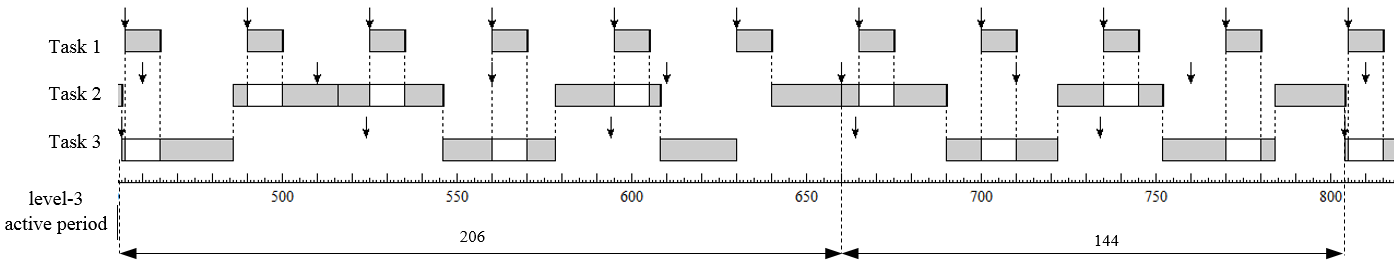
\includegraphics[width=1.1\linewidth]{figures/bcrt_ex1}
	\caption{The shortest response time of task $\tau_3$ occurs in the first job of the first level-3 active period.}
	\label{fig:bcrt1}
\end{figure}


\begin{fact}
	A task $\tau_l$ with a lower priority than a task $\tau_i$ can also affect the best-case response time of $\tau_i$ whenever $\tau_l$'s threshold $\theta_l$ is larger than or equal to $\tau_i$'s priority $\pi_i$, i.e. $\theta_i \geq \pi_i$.
\end{fact}

Further experiments suggest that this fact is probably not true. Probably a lower priority blocking task cannot affect the \textit{best-case response time} of a higher priority task $\tau_i$.

\section{Further results}

\begin{fact}
	In general, the \textit{best-case response time} is not necessarily found when the activation of all higher priority tasks that can preempt a task $\tau_i$ coincides with the completion of a job of $\tau_i$.
\end{fact}

Consider the taskset presented in Table \ref{tab:taskset2}. In Figure \ref{fig:fact5_1} a schedule is shown where the activation of higher priority tasks $\tau_1$ and $\tau_2$ coincides with the completion of a job of $\tau_4$ at time $t=736$. As can be seen, the shortest response time for $\tau_4$ under this schedule is assumed by the job activated at time $t=560$ with a response time of 32. However, this is not the \textit{best-case response time} for $\tau_4$. Figure \ref{fig:fact5_2} shows a schedule for $\mathpzc{T}_{\ref{tab:taskset2}}$ where a response time of $R_4=27$ for task $\tau_4$ is found at time $t=709$. 
\begin{table}[H]
	\center
	\caption{Task set $\mathpzc{T}_{\ref{tab:taskset2}}$.}
	\label{tab:taskset2}
	\begin{tabular}{c c c c c | c c}
		\hline 
		& $T_i$ & $WC_i=BC_i$ & $\pi_i$ & $\theta_i$ &  $wl_i$ & $BR_i$\\ 
		\hline 
		$\tau_1$& 35 & 5  & 4 & 4 &  1 & 5\\ 
		$\tau_2$& 35 & 5  & 3 & 3 &  1 & 5\\ 
		$\tau_3$& 50 & 20 & 2 & 2 &  2 & 20\\ 
		$\tau_4$& 70 & 22 & 1 & 2 &  5 & 27\\
		\hline 
	\end{tabular}
	\small
	\item The \textit{least common multiple} of the periods is 350 and $U^{\mathpzc{T_{\ref{tab:taskset2}}}}=1$.
\end{table} 

\begin{figure}[H]
	\centering
	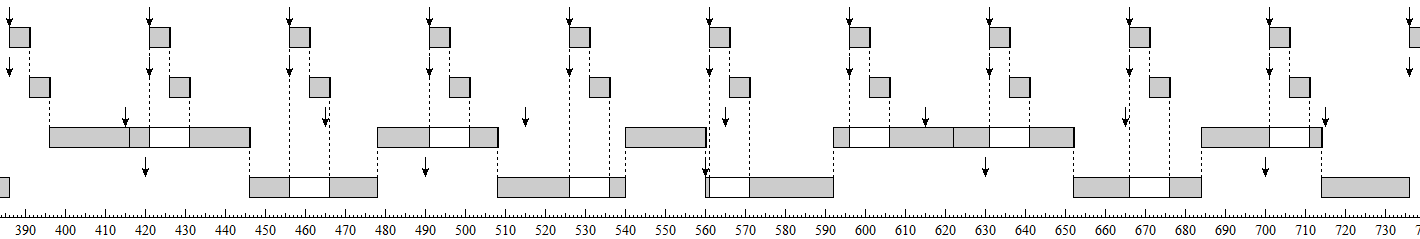
\includegraphics[width=1.1\linewidth]{figures/fact5_1}
	\caption{Simultaneous release of preemptive tasks coincides with the completion of a job of task $\tau_4$ at time 736. The phases used to construct this schedule are $\phi_1 = \phi_2 = 1$, $\phi_3 = 15$, and $\phi_4 = 0$.}
	\label{fig:fact5_1}
\end{figure}

\begin{figure}[H]
	\centering
	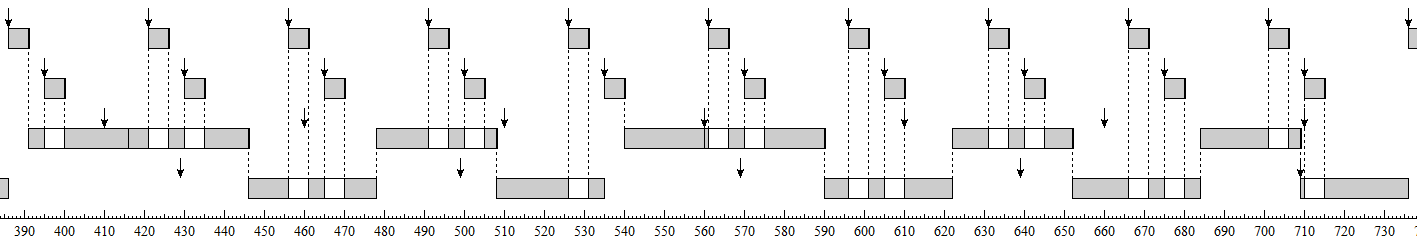
\includegraphics[width=1.1\linewidth]{figures/fact5_2}
	\caption{Schedule for $\mathpzc{T}_{\ref{tab:taskset2}}$ where the \textit{best-case response time} ($BR_4 = 27$) for $\tau_4$ is assumed at time $t=709$. The phases used to construct this schedule are $\phi_1 = 1$, $\phi_2 = \phi_3 = 10$, and $\phi_4 = 9$.}
	\label{fig:fact5_2}
\end{figure}

\begin{fact}
	A higher priority task that cannot preempt a task $\tau_i$ can provoke that the completion of task $\tau_i$ could never occur simultaneously with the release of all its higher priority preemptive tasks.
\end{fact}

Consider the task-set $\mathpzc{T}_{\ref{tab:taskset3}}$ presented in Table \ref{tab:taskset3}. Figure \ref{fig:fact6_1} shows a schedule only considering tasks $\tau_1$ and $\tau_3$  of $\mathpzc{T}_{\ref{tab:taskset3}}$ where the activation of the highest priority task $\tau_1$ coincides with the completion of task $\tau_3$. However, this situation cannot be assumed when considering also $\tau_2$. Figure \ref{fig:fact6_2} shows that as soon as $\tau_2$ is introduced in the schedule, task $\tau_3$ will always experience one preemption by $\tau_1$. Note that the first job of $\tau_2$ in Figure \ref{fig:fact6_2} delays the start time of the first job of $\tau_3$; hence, causing the completion of $\tau_3$ to not occur simultaneously with the activation of $\tau_1$.

\begin{table}[H]
	\center
	\caption{Task set $\mathpzc{T}_{\ref{tab:taskset3}}$.}
	\label{tab:taskset3}
	\begin{tabular}{c c c c c | c c}
		\hline 
		& $T_i$ & $WC_i=BC_i$ & $\pi_i$ & $\theta_i$ &  $wl_i$ & $BR_i$\\ 
		\hline 
		$\tau_1$& 80  & 20  & 3 & 3 &  1 & 20\\ 
		$\tau_2$& 30  & 15  & 2 & 2 &  2 & 15\\ 
		$\tau_3$& 240 & 50  & 1 & 2 &  1 & 70\\ 
		\hline 
	\end{tabular}
	\small
	\item The \textit{least common multiple} of the periods is 240 and $U^{\mathpzc{T_{\ref{tab:taskset2}}}} \approx 0.96$.
\end{table} 

\begin{figure}[H]
	\centering
	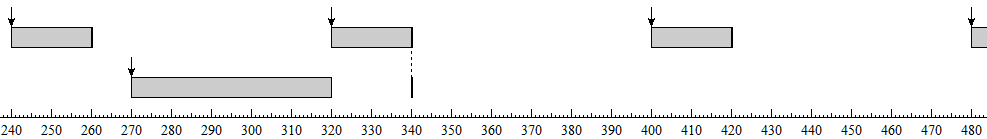
\includegraphics[width=0.9\linewidth]{figures/fact6_1}
	\caption{Schedule of task-set $\mathpzc{T}_{\ref{tab:taskset3}} \textbackslash \{\tau_2\}$. The phases used to construct this schedule are $\phi_1 = 0$ and $\phi_3 = 30$.}
	\label{fig:fact6_1}
\end{figure}

\begin{figure}[H]
	\centering
	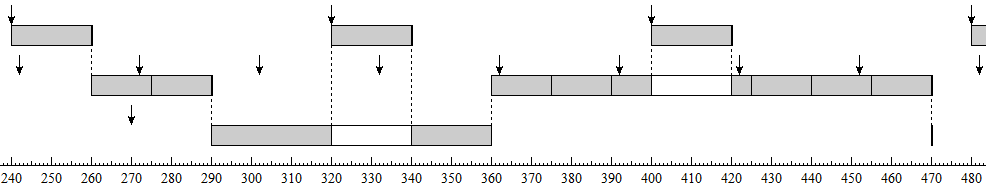
\includegraphics[width=0.9\linewidth]{figures/fact6_2}
	\caption{Schedule of task-set $\mathpzc{T}_{\ref{tab:taskset3}}$. The phases used to construct this schedule are $\phi_1 = 0$, $\phi_2 = 2$ and $\phi_3 = 30$.}
	\label{fig:fact6_2}
\end{figure}

\subsection{Blocking tasks}

\begin{fact}
	A lower priority task that can block the execution of a task $\tau_i$ cannot affect the \textit{best-case response time} of $\tau_i$.
\end{fact}

Consider task-set $\mathpzc{T}_{\ref{tab:taskset4}}$ described in Table \ref{tab:taskset4}. Figure \ref{fig:fact7_1} shows an schedule for such a task-set, but only considering tasks $\tau_1$ and $\tau_2$. As can be seen, the \textit{best-case response time} $BR_2=50$ for task $\tau_2$ is assumed in the schedule. Introducing the blocking task $\tau_3$ could affect the response time of task $\tau_2$ as shown in Figure \ref{fig:fact7_2}. However, it is always possible to re-schedule a blocking task in such a way that it does not affect the \textit{best-case response time} of its higher priority tasks. Figure \ref{fig:fact7_3} shows the task-set $\mathpzc{T}_{\ref{tab:taskset4}}$ scheduled in such a way that the \textit{best-case response time} for task $\tau_2$ is assumed.

\begin{table}[H]
	\center
	\caption{Task set $\mathpzc{T}_{\ref{tab:taskset4}}$.}
	\label{tab:taskset4}
	\begin{tabular}{c c c c c | c c}
		\hline 
		& $T_i$ & $WC_i=BC_i$ & $\pi_i$ & $\theta_i$ &  $wl_i$ & $BR_i$\\ 
		\hline 
		$\tau_1$& 80  & 20  & 3 & 3 &  1 & 20\\
		$\tau_2$& 240 & 50  & 2 & 2 &  1 & 50\\ 
		$\tau_3$& 30  & 15  & 1 & 2 &  8 & 15\\ 
		\hline 
	\end{tabular}
	\small
	\item The \textit{least common multiple} of the periods is 240 and $U^{\mathpzc{T_{\ref{tab:taskset2}}}} \approx 0.96$.
\end{table} 

\begin{figure}[H]
	\centering
	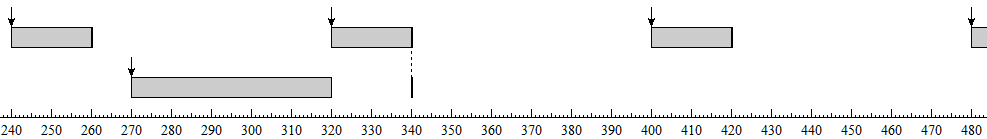
\includegraphics[width=0.9\linewidth]{figures/fact6_1}
	\caption{Schedule of taskset $\mathpzc{T}_{\ref{tab:taskset4}} \textbackslash \tau_3$. The phases used to construct this schedule are $\phi_1 = 0$ and $\phi_2 = 30$.}
	\label{fig:fact7_1}
\end{figure}

\begin{figure}[H]
	\centering
	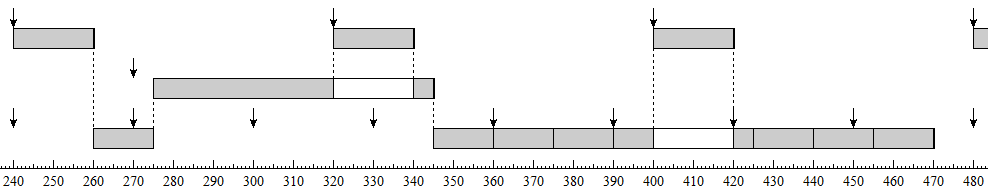
\includegraphics[width=0.9\linewidth]{figures/fact7_2}
	\caption{Schedule of task-set $\mathpzc{T}_{\ref{tab:taskset4}}$. The phases used to construct this schedule are $\phi_1 = \phi_3 = 0$ and $\phi_2 = 30$.}
	\label{fig:fact7_2}
\end{figure}

\begin{figure}[H]
	\centering
	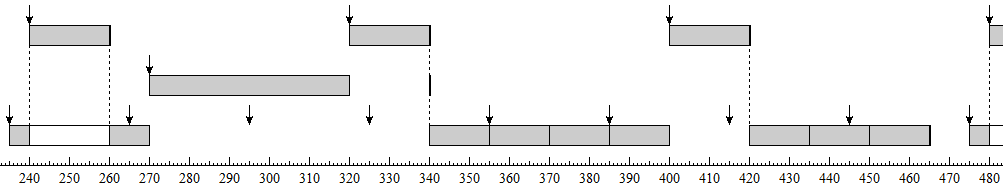
\includegraphics[width=0.9\linewidth]{figures/fact7_3}
	\caption{Schedule of task-set $\mathpzc{T}_{\ref{tab:taskset4}}$ where the \textit{best-case response time} for task $\tau_2$ is assumed. The phases used to construct this schedule are $\phi_1 = 0$ , $\phi_3 = 25$ and $\phi_2 = 30$.}
	\label{fig:fact7_3}
\end{figure}

\section{BCHT for FPTS}

Given a task-set $\mathpzc{T}$, Algorithm 1 shows a procedure to derive a less pessimistic lower bound for the \textit{best-case hold time} of a task $\tau_i$. Table \ref{tab:terminology} explain the terminology for the variables used in the algorithm. Furthermore, function $BI_i(y,PA_d)$ returns the the largest positive solution satisfying

\begin{align}
x = y + \sum\limits_{h:\pi_h > \theta_i} \Big( \Big\lceil  \dfrac{x}{T_h}\Big\rceil -1 \Big)^+  BC_h + \sum\limits_{d:\theta_i \geq \pi_d \pi_i} \Big( \Big\lceil  \dfrac{x-PA_d}{T_d}\Big\rceil -1 \Big)^+  BC_d,
\end{align}

\noindent
where the notion $w^+$ stands for $\max(w,0)$.

\begin{table}[H]
	\center
	\caption{Terminology.}
	\label{tab:terminology}
	\begin{tabular}{|c | p{9cm}|}
		\hline
		Name & Descriptions \\ 
		\hline 
		\hline
		$HLB^{init}_i$& Initial lower bound. This is the \textit{best-case hold time} of task $\tau_i$ when considering only preemptive tasks.\\
		\hline
		$LB_i$& Lower bound of the \textit{best-case hold time} if $\tau_i$; $BH_i > LB_i.$\\
		\hline
		$UB_i$& Upper bound in hold time when pushing the activation of delaying tasks. \\ 
		\hline
		$PI_i$ & Push interval of delaying tasks relative to $LB_i$.   \\ 
		\hline
		$DI_i$ & Delay interval of task $\tau_i$ is the time interval in which delaying tasks can affect the hold time.\\
		\hline 
	\end{tabular}
	%\small
	%\item The \textit{least common multiple} of the periods is 240 and $U^{\mathpzc{T_{\ref{tab:taskset2}}}} \approx 0.96$.
\end{table} 

\begin{algorithm}[H]
	\caption{Algorithm to derive a tighter lower bound for the \textit{best-case hold time} of task $\tau_i$.}\label{euclid}
	\begin{algorithmic}[1]
		\Procedure{\textit{HLB}$_i$}{$\mathpzc{T}$}
		\State $HLB^{init}_i = BI_i(BC_i,\infty)$;
		\State $PI_i = -\delta$;
		\State $LB_i = HLB^{init}_i + PI_i$;
		\State $UB_i = BI_i(BC_i,LB_i)$;
		\If {$UB_i > HLB^{init}_i$}
		\State $LB_i = HLB^{init}_i$;
		\EndIf {\textbf{end if}}
		\While {$UB_i > HLB^{init}_i$}
		\State $DI_i = UB_i - LB_i$;
		\State $PI_i = \min \limits_{d:\theta_i \geq \pi_d > \pi_i} (DI_i \mod T_d);$
		\State $LB_i = LB_i + PI_i$;
		\State $UB_i = BI_i(BC_i,LB_i)$;
		\EndWhile{\textbf{end while}}
		\State \Return $LB_i$; 
		\EndProcedure
	\end{algorithmic}
\end{algorithm}

In order to illustrate how the algorithm works, consider the task-set $\mathpzc{T}_{\ref{tab:taskset5}}$ described in Table \ref{tab:taskset5}. Figure \ref{fig:bcht_1} shows the notions after performing Algorithm 1 to calculate $HLB_4=55$. Note that in Figure \ref{fig:bcht_1}, the second job of $\tau_3$ activated at time $t=30$, namely $\iota_{3,2}$, does not start. This is to illustrate that the \textit{best-case hold time} of $\tau_4$ should be long enough in order to delay the start time of $\iota_{3,2}$, i.e. $BH_4 > HLB_4$. If this condition is not met, the job $\iota_{3,2}$ will start and delay the start time of $\tau_4$. As a consequence, the job of $\tau_4$ will experience preemptions by the higher priority tasks activated at time $t=85$.

\begin{table}[H]
	\center
	\caption{Task set $\mathpzc{T}_{\ref{tab:taskset5}}$.}
	\label{tab:taskset5}
	\begin{tabular}{c c c c c | c c c c}
		\hline 
		& $T_i$ & $WC_i=BC_i$ & $\pi_i$ & $\theta_i$ &  $wl_i$ & $BR_i$ & $HLB_i$ & $HLB^{init}_i$\\ 
		\hline 
		$\tau_1$& 80  & 14  & 4 & 4 &  1 & 14 & &\\
		$\tau_2$& 80  & 6   & 3 & 3 &  1 & 6  & &\\ 
		$\tau_3$& 30  & 15  & 2 & 2 &   & 15  & &\\ 
		$\tau_4$& 240 & 50  & 1 & 2 &   & 56  & 55& 50\\
		\hline 
	\end{tabular}
	\small
	\item The \textit{least common multiple} of the periods is 240 and $U^{\mathpzc{T_{\ref{tab:taskset5}}}} \approx 0.96$.
\end{table}

\begin{figure}[H]
	\centering
	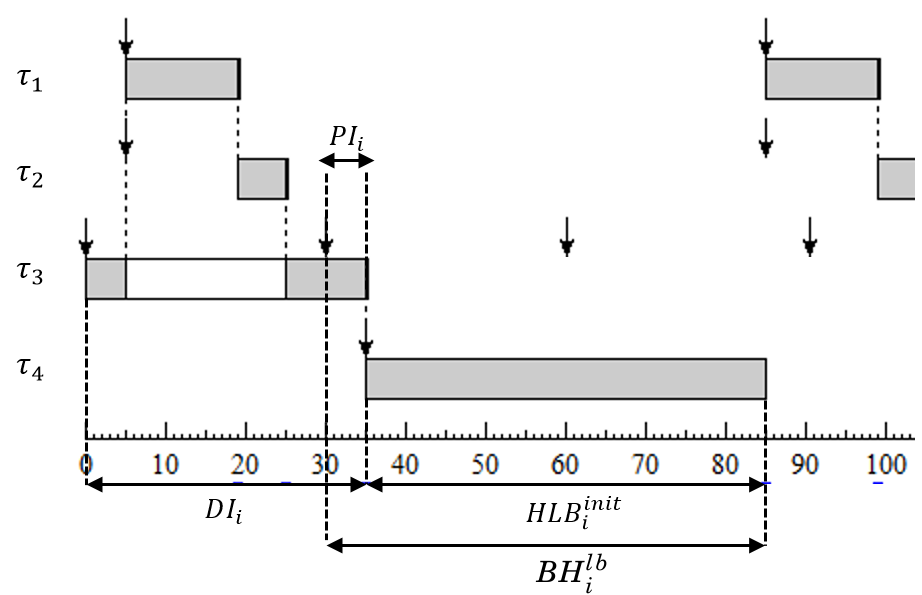
\includegraphics[width=0.7\linewidth]{figures/bcht_1}
	\caption{Schedule of task-set $\mathpzc{T}_{\ref{tab:taskset5}}$ with the notions described in Table \ref{tab:terminology}.}
	\label{fig:bcht_1}
\end{figure}

Note that the only way for the job of task $\tau_4$ to have a hold time higher than $HLB_4=55$ is by experiencing preemption by either task $\tau_1$, $\tau_2$ or both. Since $\tau_2$ has a \textit{best-case execution time} $BC_2=6$, we can choose this task to preempt $\tau_4$ and the condition will be met because $HLB^{init}_i+BC_2= 56$ which is higher than $HLB_i = 55$. This is indeed the \textit{best-case hold time} because if we would choose $\tau_1$ to preempt $\tau_4$, the resulting hold time would be $HLB^{init}_i+BC_1= 64$. Figure \ref{fig:bcht_2} shows the schedule where the \textit{best-case hold time} for task $\tau_4$ is assumed.

\begin{figure}[H]
	\centering
	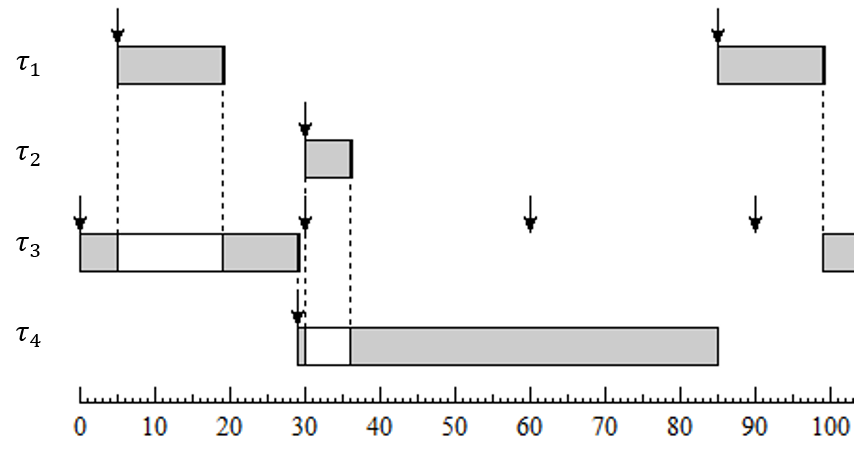
\includegraphics[width=0.7\linewidth]{figures/bcht_2}
	\caption{Schedule of task-set $\mathpzc{T}_{\ref{tab:taskset5}}$ where the \textit{best-case hold time} of task $\tau_4$ is assumed ($BH_4 = 56$).}
	\label{fig:bcht_2}
\end{figure}

\section{BCRT lower bound for FPTS}
Given a task-set $\mathpzc{T}$ of strictly periodic tasks, Algorithm 2 shows a procedure to derive a lower bound for the \textit{best-case response time} of a task $\tau_i$. The algorithm first determine a lower bound for the hold time and the activation $AD_i$ of the delaying tasks of $\tau_i$ is set to this value in Line 2. In Line 3, the $BR^{lb}_i$ is initialized with some upper bound. A lower bound candidate is derived in Line 5 using a similar approach as for the \textit{best-case response time} analysis for FPPS. The purpose of the outer max is to make sure that $BR^{lb}_i$ is at least the same as the activation of delaying tasks $AD_i$. In case that $BR^{lb}_i$ is higher than $AD_i$, Lines 7 to 9 push the activation for the delaying tasks in order to allow to reduce $BR^{lb}_i$ in the next iteration. More precisely, the job $k^{tight}$ of task $\tau_i$ that induces some delay on the start time of the job experiencing the optimal instant is determined in Line 7. Moreover, Lines 8 and 9 determine the time the activation of delaying tasks should be pushed at an earlier moment, to prevent job $k^{tight}$ from inducing some blocking. At this point, if the new value of $AD_i$ exceeds the current $BR^{lb}_i$, then it is not beneficial to push the activation of delaying tasks to reduce the \textit{best-case response time}; hence, the algorithm terminates.

\begin{table}[H]
	\center
	\caption{Terminology.}
	\label{tab:terminology}
	\begin{tabular}{|c | p{9cm}|}
		\hline
		Name & Descriptions \\ 
		\hline 
		\hline
		$AD_i$& Activation of delaying tasks relative to the optimal instant.\\
		\hline
		$DI_i$& Time interval from the activation of job $k$ of $\tau_i$ that provokes a delay on the start time of the job experiencing the optimal instant to the activation of delaying tasks.\\
		\hline 
	\end{tabular}
	%\small
	%\item Add extra caption.
\end{table} 

\begin{algorithm}[H]
	\caption{Algorithm to derive a lower bound for the \textit{best-case response time} of task $\tau_i$.}\label{euclid}
	\begin{algorithmic}[1]
		\Procedure{\textit{bcrtLowerBound}}{$\mathpzc{T}$,$i$}
		\State $AD_i \gets HLB(\mathpzc{T},i)$;
		\State $BR^{lb}_i \gets \infty$;
		\While {$BR^{lb}_i > AD_i$}
		\State $BR^{lb}_i \gets \max\{ AD_i, \max \limits_{2 \leq k \leq wl_i} (BI_i(k \cdot BC_i, AD_i) - (k-1)T_i) \}$;
		\If {$BR^{lb}_i > AD_i$}
		\State $k^{tight} \gets$ the maximum job $k$ with $2 \leq k \leq wl_i$ that leads to $BR^{lb}_i$;
		\State $DI_i \gets BI_i(k^{tight} \cdot BC_i, AD_i) - AD_i$;
		\State $AD_i \gets \min \limits_{d:\theta_i \geq \pi_d > \pi_i} (DI_i \mod T_d) + AD_i$
		\EndIf {\textbf{end if}}
		\EndWhile{\textbf{end while}}
		\State \Return $BR^{lb}_i$; 
		\EndProcedure
	\end{algorithmic}
\end{algorithm}

\subsection{An example}
Consider the set of tasks $\mathpzc{T}_{\ref{tab:ts_example}}$ with characteristics as described in Table $\ref{tab:ts_example}$. We will apply Algorithm 2 to derive a lower bound for the \textit{best-case response time} $BR_4$ of task $\tau_4$. Figure \ref{fig:bcrt_lb_ex1} shows an example of how each variable of the algorithm would be represented in a schedule after the first iteration. As can be seen, $AD^{(0)}_4=22$ represents the initial value of $AD_4$, and it is equal to the hole time of the last job of $\tau_4$. Furthermore, the job of $\tau_4$ activated at time $t=560$ denoted as $k^{tight}$ is the one that leads to the $BR^{lb (1)}_4=36$. Based on this, the algorithm then determines the value $AD^{(1)}_4=26$ that would allow to push the phase of $\phi_4$ further in order to reduce the \textit{best-case response time} of $\tau_4$. Note that $BR^{lb (1)}_4$ is larger than $AD^{(1)}_4$; hence, the algorithm will continue with the next iteration.

\begin{table}[H]
	\center
	\caption{Task set $\mathpzc{T}_{\ref{tab:ts_example}}$.}
	\label{tab:ts_example}
	\begin{tabular}{c c c c c | c c}
		\hline 
		& $T_i$ & $WC_i=BC_i$ & $\pi_i$ & $\theta_i$ &  $wl_i$ & $BR_i$\\ 
		\hline 
		$\tau_1$& 35 & 5  & 4 & 4 &  1 & 5\\ 
		$\tau_2$& 35 & 5  & 3 & 3 &  1 & 5\\ 
		$\tau_3$& 50 & 20 & 2 & 2 &  2 & 20\\ 
		$\tau_4$& 70 & 22 & 1 & 2 &  5 & 27\\
		\hline 
	\end{tabular}
	\small
	\item The \textit{least common multiple} of the periods is 350 and $U^{\mathpzc{T_{\ref{tab:ts_example}}}}=1$.
\end{table}

\begin{figure}[H]
	\centering
	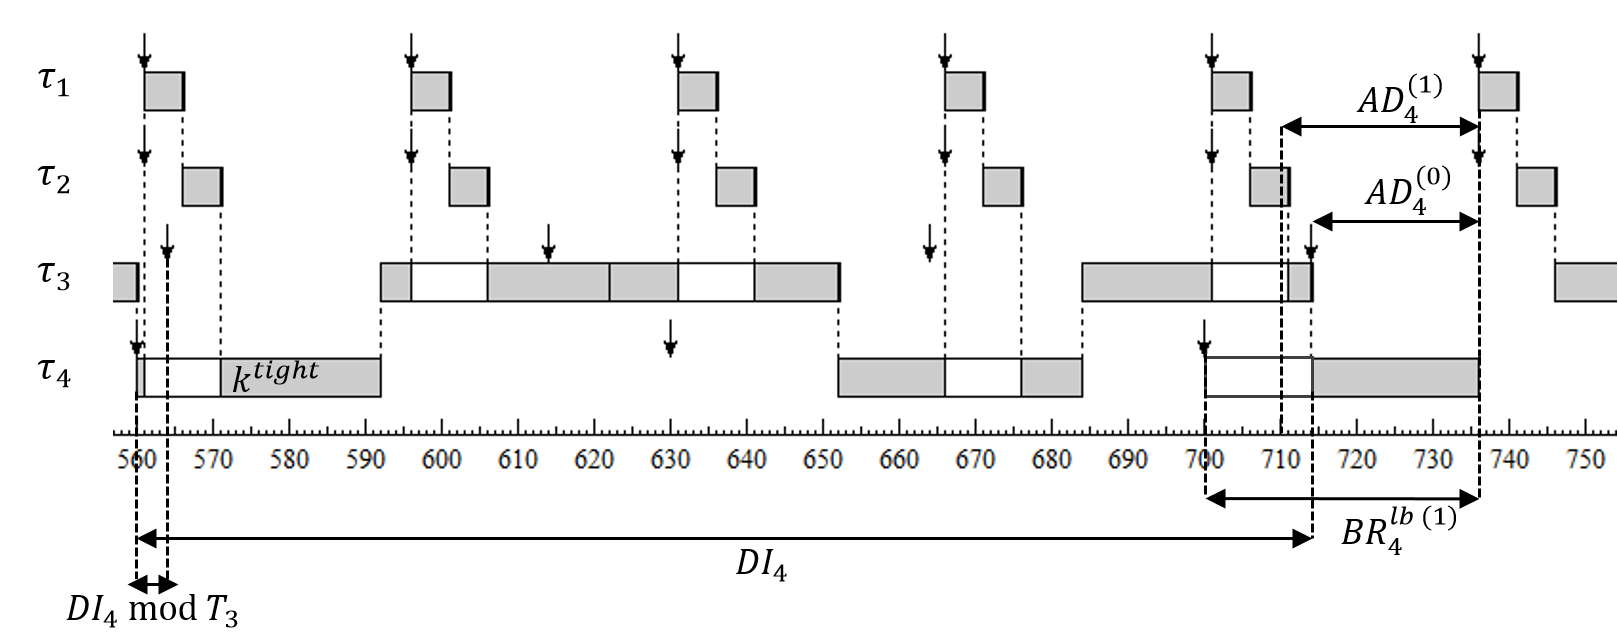
\includegraphics[width=1\linewidth]{figures/bcrt_lb_ex1.PNG}
	\caption{Example after the first iteration of $bcrtLowerBound(\mathpzc{T}_{\ref{tab:ts_example}},4)$. }
	\label{fig:bcrt_lb_ex1}
\end{figure}

Figure \ref{fig:bcrt_lb_ex2} shows the schedule in the second iterations of $bcrtLowerBound(\mathpzc{T}_{\ref{tab:ts_example}},4)$. As can be seen, the activations of the delaying task $\tau_3$ was pushed to an earlier moment in time, allowing to decrease the response time of the last job. At this point $BR^{lb(2)}_4 = AD^{(2)}_4 = 26$; hence, the algorithm will terminate because there is no previous job restricting the response time of the last job.

\begin{figure}[H]
	\centering
	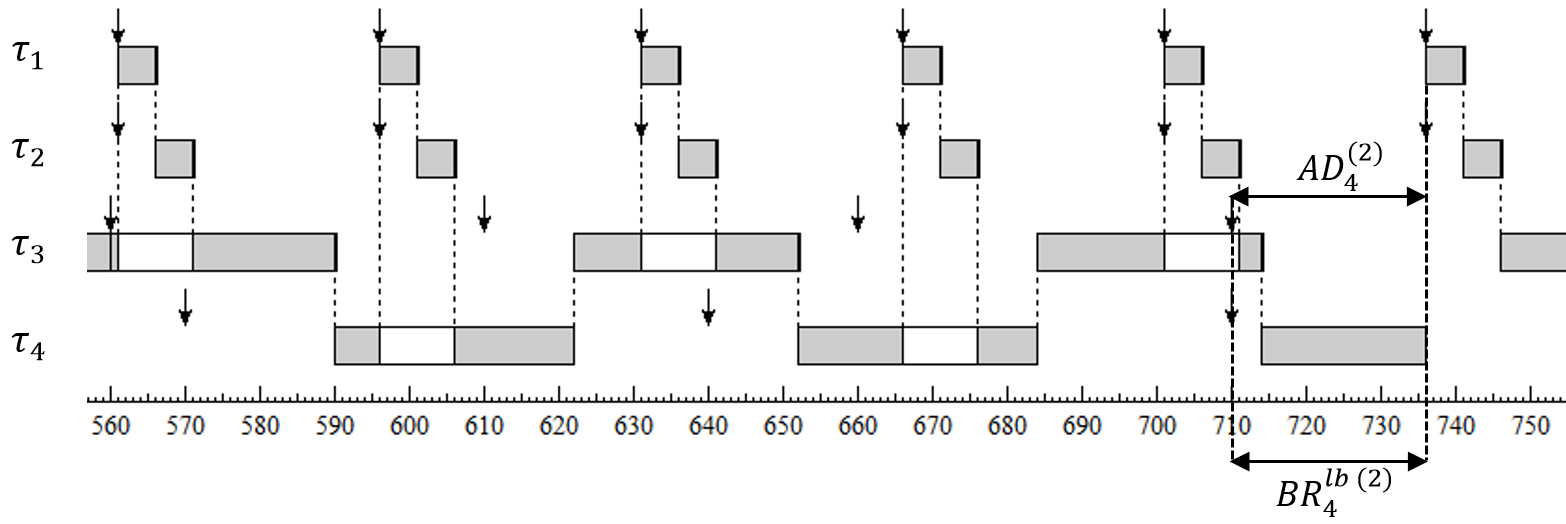
\includegraphics[width=1\linewidth]{figures/bcrt_lb_ex2.PNG}
	\caption{Example after the second iteration of $bcrtLowerBound(\mathpzc{T}_{\ref{tab:ts_example}},4)$. }
	\label{fig:bcrt_lb_ex2}
\end{figure}

We conclude that  $BR^{lb}_4 = 26$ is a proper lower bound for the \textit{best-case response time} of $\tau_4$.

\begin{thebibliography}{10}
	
	\bibitem{WS99}
	Y. Wang, and M. Saksena.
	Scheduling fixed-priority tasks with preemption thresholds.
	In Proc. 6th International Conference on Real-Time Computing Systems and Applications (RTCSA), December 1999.	
	
	\bibitem{BHKL12}
	R.J. Bril, M. van den Heuvel, U. Keskin, and J. Lukkien.
	Generalized fixed-priority scheduling with preemption thresholds.
	In Proc. 24th Euromicro Conference on Real-Time Systems (ECRTS), July 2012.
	
	\bibitem{BHL13}
	R.J. Bril, M.M.H.P. v.d. Heuvel, and J.J. Lukkien.
	Improved feasibility of fixed-priority scheduling with deferred preemption using preemption thresholds for preemption points.
	In Proc. 21st International Conference on Real-Time Networks and Systems (RTNS), ACM, pp. 225-264, October 2013.
	
	\bibitem{BFV08}
	R.J. Bril, G. Fohler, and W.F.J. Verhaegh. 
	Execution times and execution jitter of real-time tasks under fixed-priority preemptive scheduling. 
	Technical Report CSR 08-27, TU/e, The Netherlands, Oct. 2008. \url{http://www.win.tue.nl/~mholende/cantata/publications/BCG-WiP-ECRTS09-final.pdf}
	
	\bibitem{BLM13}
	R.J. Bril, J.J. Lukkien, and R.H. Mak.
	Best-case response times and jitter analysis of real-time tasks with arbitrary deadlines.
	In Proc. 21st International Conference on Real-Time Networks and Systems (RTNS), ACM, pp. 193-202, October 2013.
	
	\bibitem{C99}
	A. Cervin. 
	Improved Scheduling of Control Tasks.
	In Proc. 11th Euromicro Conference on Real-Time Systems (ECRTS), York, England, pp 4 - 10, 09 Jun 1999. 
	
	\bibitem{CRA99} 
	A. Crespo, I. Ripoll, and P. Albertos. 
	Reducing Delays in RT Control: The Control Action Interval. 
	In 14th IFAC World Congress on Automatic Control. Elsevier Science. p. 0. 1999.
	
	\bibitem{BC07} 
	G. Butazzo and A. Cervin. 
	Comparative Assessment and Evaluation of Jitter Control Methods. 
	In Proc. 15th International Conference on Real-Time and Network Systems (RTNS), Nancy, France, March 29-30, 2007.
	
	\bibitem{LCBRC06}
	M. Lluesma, A. Cervin, P. Balbastre, I. Ripoll, and A. Crespo.
	Jitter evaluation of real-time control systems.
	In Proceedings of the 12th IEEE International Conference on Embedded and Real-Time Computing Systems and Applications, 2006, pp. 257-260.
	
	\bibitem{THLT06}
	Y. Tian, Q. Han, D. Levy, and M. Tade. 
	Reducing Control Latency and Jitter in Real-Time Control.
	Asian Journal of Control, Vol. 8, No. 1, pp. 72-75, March 2006.
	
	\bibitem{BRVC04}
	P. Balbastre, I. Ripoll, J. Vidal, and A. Crespo.
	A task model to reduce control delays.
	Real-Time Syst., vol. 27, no. 3, pp. 215-236, Sep. 2004.
	
	\bibitem{BBGL99}
	S. Baruah, G. Buttazzo, S. Gorinsky, and G. Lipari. 
	Scheduling periodic task systems to minimize output jitter. 
	In Proc. International Conference on Real-Time Computing Systems and 
	Applications, pages 62-69, Hong Kong, December 1999.
	
	\bibitem{HHL10}
	S. Hong, X. Hu, and M. Lemmon.
	Reducing delay jitter of real-time control tasks through adaptive deadline adjustments.
	In Euromicro Conference on Real-Time Systems (ECRTS), 2010, pp. 229-238.
	
	\bibitem{MVFF01}
	P. Marti, R. Villa, J.M. Fuertes, G. Fohler. 
	On Real-Time Control Task Schedulability. 
	In European Control Conference (ECC), Porto, Portugal, 4-7 September 2001.
	
	\bibitem{MFFR01}
	P. Marti, J.M. Fuertes, G. Fohler, and K. Ramamritham. 
	Jitter Compensation for Real-Time Control System. 
	In Proceedings of the 22nd IEEE Real-Time Systems Symposium, pp 39-48, 2001.
	
	\bibitem{MFF01}
	P. Marti, J.M. Fuertes, G. Fohler. 
	Sampling Jitter Compensation in Real-time Control Systems. 
	In Proceedings of the 22nd IEEE Real-Time Systems Symposium (RTSS 2001), 
	London, UK, 2-6 December 2001.
	
	\bibitem{WB09}
	Y. Wu and M. Bertogna.
	Improving task responsiveness with limited preemptions.
	In Proc. 14th IEEE Int. Conf. Emerging Technol. Factory Autom. (ETFA 2009), 
	Mallorca, Spain, Sep. 2009.
	
	\bibitem{L90}
	J.P. Lehoczky.
	Fixed Priority Scheduling of Periodic Task Sets with Arbitrary Deadline.
	In Proceeding of the 11th IEEE Real-Time System Symposium (RTSS 1990), pp 201-209, December 1990.
	
	\bibitem{HKL91}
	M. G. Harbour, M. H. Klein, and J. P. Lehoczky. 
	Fixed priority scheduling periodic tasks with varying execution priority.
	Real-Time Systems Symposium, pages 116-128, December 1991.
	
	\bibitem{LL73}
	C. Liu and J. Layland.
	Scheduling algorithms for multiprogramming in a real-time environment.
	In Journal of the ACM, vol. 20, no. 1, pp. 46-61, January 1973.	
	
	\bibitem{KBL10}
	U. Keskin, R.J. Bril and J. Luikkien.
	Exact response-time analysis for fixed-priority preemption-threshold scheduling.
	In Proc. IEEE Conference on Emerging Technologies and Factory Automation (ETFA), Working-Progress Session, September 2010.
	
	\bibitem{BAHDB17}
	R.J. Bril, S. Altmeyer, M.M.H.P. van den Heuvel, R.I. Davis, and M. Behnam.
	Fixed priority scheduling with pre-emption thresholds and cache-related pre-emption delays: integrated analysis and evaluation.
	In Real-Time Systems, 31 January 2017.	
	doi:10.1007/s11241-016-9266-z
	
	\bibitem{GRASP}
	Mike Holenderski, Martijn M. H. P. van den Heuvel, Reinder J. Bril and Johan J. Lukkien.
	Grasp: Tracing, Visualizing and Measuring the Behavior of Real-Time Systems.
	In International Workshop on Analysis Tools and Methodologies for Embedded and Real-time Systems (WATERS), July 2010.
	
	
\end{thebibliography}
\end{document}

